\section{Model Component} \label{sc:model_component}
Based on the analysis of the problem domain (see \autoref{ch:problemdomain}), through the class diagram, event table, and state charts, the model component of the system has been constructed.
\par
The model component, mentioned in \autoref{sc:component_architecture}, has been constructed by first looking at the original class diagram from the problem domain (see \autoref{fig:FirstPDClassDiagram}). Then additional classes, attributes, and structures have been added to support the mentioned events and the desired functionality of the system. The result is an updated class diagram that contains attributes, operations, and additional classes and structures.
\par
First the \textit{Employee} and \textit{Admin} classes need a revision. The \textit{Employee} class has been used to keep track of the employees in the system. This has been done to keep track of who are in possession of what assets, which the \textit{Tag} class can already do. The other function of the \textit{Employee} class is to know which employees are admins and which are not. This function has been handled in a class in the function component, which will be explained in a later section (see \autoref{sc:function_component}), and therefore the \textit{Employee} and \textit{Admin} classes have become obsolete.

\subsection{Additional classes}
Based on the events and desired functionality of the system, the following classes have been added to the class diagram. 

% \subsubsection{Tag}
% The \textit{Asset} class has the attribute 'Asset State' and the function 'Asset Acquired()', which can both be replaced by a class named \textit{Tag}. With the \textit{Tag} class, the \textit{Loan} will also be obsolete, as the employee currently borrowing the asset can be tagged onto the asset. The \textit{Tag} class will contain information about the asset, as well as timestamps for the tag's creation, last update and deletion. It will also be used to search through the assets. This \textit{Tag} class and tagging functionality have been requested by the customer. 

% \subsubsection{Tag relation}
% The \textit{Tag relation} class has been added to represent a connection between an asset and a tag, as an asset can have multiple tags related to it and a tag can be related to multiple assets.

% \subsubsection{Department}
% To more easily divide the assets and avoid cluttering the user with assets, a new class \textit{Department} has been added to the class-diagram. A department will have a name and contain a number of assets. An employee have a standard department, which they will be located in, when they open the application. The department can be change in the system by the employee, to see assets in another department, so the standard department will only be used as a starting point. A department also has timestamps for its creation and last update.

\subsubsection{Field}
To simplify the process of adding an asset to the system, the page for adding and editing an asset should only contain the relevant information. This helps with decluttering of the page and supports the wish to only fill in relevant information intuitively. To make this easier, the \textit{Field} class is introduced. The \textit{Field} class can be contained by both tags and assets. If a field is contained by a tag and that tag is attached to an asset, the field is added to the asset as well. Fields only exists on an asset or a tag and never alone.
\par
A field contains the following attributes:
\begin{itemize}
    \item ID
    \item Name
    \item Type of the input, which can be: a textbox, a textarea, a number, a date, or a checkbox. \todo[inline]{Add potential additional field types}
    \item Content, which will hold the value set by the user (will never be set on a tag)
    \item Required, which defines whether or not the field must be filled in before saving the asset.
    \item \textit{Default value of the field, if it is connected to a tag, when it is added to an asset.}\newline This is only available on the fields added to a tag (see \autoref{fig:FieldWithAttributes}).
\end{itemize}
\begin{figure}[H]
    \centering
    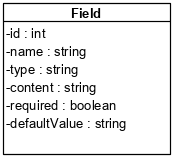
\includegraphics[width=0.28\textwidth]{figures/Classes/FieldAttributes.png}
    \caption{Overview of the \textit{Field} class with attributes}
    \label{fig:FieldWithAttributes}
\end{figure}
% If the field is added to a tag, the field will appear on the asset as soon as it has been tagged with the given tag. When the field is added to a tag, the user can set a default value, which the field will have when an asset is tagged with the tag.
% \par
% Fields added directly to an asset does not give the opportunity to set a default value.

\subsubsection{Comment}
To better organize and structure the employee's comments on an asset, a \textit{Comment} class has been introduced. A comment can be attached to an asset and contains the id of the asset, the id of the employee whom the comment was added by, a comment text, and timestamps for its creation and last update (see \autoref{fig:CommentWithAttributes}).
\begin{figure}[H]
    \centering
    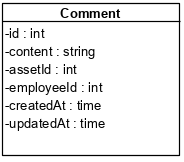
\includegraphics[width=0.28\textwidth]{figures/Classes/CommentAttributes.png}
    \caption{Overview of the \textit{Comment} class with attributes}
    \label{fig:CommentWithAttributes}
\end{figure}

\subsubsection{FieldContainer}
To ensure that both the asset and tag classes have a list of fields and implement the correct properties, an abstract class has been implemented called \textit{FieldContainer}. Both the asset and tag classes are specializations of this abstract class (see \autoref{fig:FieldContainer}).
\begin{figure}[H]
    \centering
    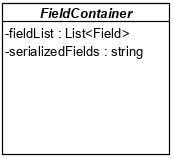
\includegraphics[width=0.28\textwidth]{figures/Classes/FieldContainer.png}
    \caption{Overview of the \textit{FieldContainer} class with attributes}
    \label{fig:FieldContainer}
\end{figure}

\subsection{Attributes}
To ensure that every event and functionality is supported, the following attributes have been added to the classes from the class diagram in the problem domain (see \autoref{fig:FirstPDClassDiagram}).

\subsubsection{Asset attributes}
An asset has an id, a name, a description, a list of fields, and timestamps for its creation, last update, and deletion. The deletion time is used for soft deletion, which works as an extra step to avoid unwanted deletes. Soft deletion works by marking an asset with a deletion date in the database, instead of removing the element from the database. This allows the asset to be recovered, if it is accidentally deleted (see \autoref{fig:AssetWithAttributes}).

\begin{figure}[H]
    \centering
    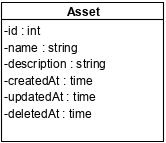
\includegraphics[width=0.28\textwidth]{figures/Classes/AssetAttributes.png}
    \caption{Overview of the \textit{Asset} class with attributes}
    \label{fig:AssetWithAttributes}
\end{figure}

\subsubsection{Department attributes}
A department has an id, a name, and a number of assets and tags. It also contains timestamps for its creation and last update (see \autoref{fig:DepartmentWithAttributes}).
\begin{figure}[H]
    \centering
    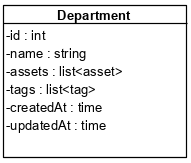
\includegraphics[width=0.28\textwidth]{figures/Classes/DepartmentAttributes.png}
    \caption{Overview of the \textit{Department} class with attributes}
    \label{fig:DepartmentWithAttributes}
\end{figure}

\subsubsection{Tag attributes}
The \textit{Tag} class will contain an id, a name, timestamps for the tag's creation and last update, and a number of fields (see \autoref{fig:TagWithAttributes}).
\begin{figure}[H]
    \centering
    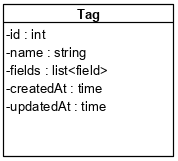
\includegraphics[width=0.28\textwidth]{figures/Classes/TagAttributes.png}
    \caption{Overview of the \textit{Tag} class with attributes}
    \label{fig:TagWithAttributes}
\end{figure}

% \subsubsection{Asset-tag relation attributes}
% The \textit{Asset-tag relation} class contains an id and the id of the asset and tag it connects.
% \begin{figure}[H]
%     \centering
%     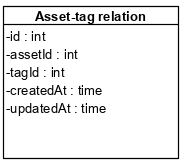
\includegraphics[width=0.5\textwidth]{figures/Classes/Asset-tagRelationAttributes.png}
%     \caption{Overview of the \textit{Asset-tag relation} class with attributes}
%     \label{fig:Asset-tagRelationWithAttributes}
% \end{figure}

These attributes and classes are accompanied by additional structures connecting the classes. These structures have been explained below.

\subsection{Structures}
The events and functions not completely supported by the previously mentioned classes and attributes will be achieved with the following structures of classes.

\subsubsection{Assets and tags can contain fields}
Both the \textit{Asset} and the \textit{Tag} classes aggregates the \textit{Field} class. An asset or a tag can contain multiple fields, but a field belongs to only one asset or one tag. To ensure that both classes have a list of fields and implement the correct properties, they both specialize the abstract class \textit{FieldContainer} (see \autoref{fig:AssetTagFieldStructure}).

\begin{figure}[H]
    \centering
    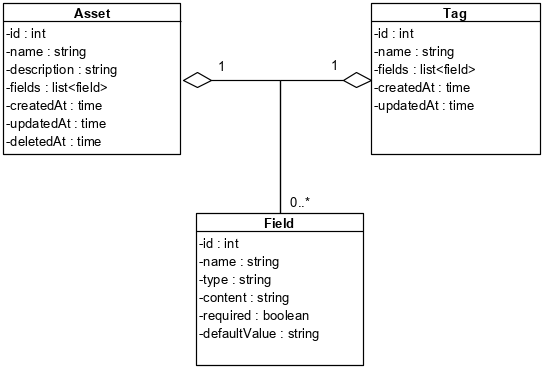
\includegraphics[width=0.8\textwidth]{figures/Structures/AssetTagFieldStructure.png}
    \caption{Overview of the structure between the \textit{Asset}, \textit{Tag}, \textit{FieldContainer}, and \textit{Field} classes}
    \label{fig:AssetTagFieldStructure}
\end{figure}

\subsubsection{An asset contains comments}
An asset can be commented on, which attaches the comment to the asset. An asset can have multiple comments, but a comment can only be attached to one asset (see \autoref{fig:AssetCommentStructure}).

\begin{figure}[H]
    \centering
    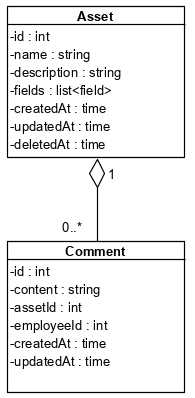
\includegraphics[width=0.25\textwidth]{figures/Structures/AssetCommentStructure.png}
    \caption{Overview of the structure connecting the \textit{Asset} and \textit{Comment} classes}
    \label{fig:AssetCommentStructure}
\end{figure}

% \subsubsection{Tag relation between asset and tag}
% Between the \textit{Tag} and \textit{Asset} classes is a many-to-many relation, which has been replaced by the class \textit{Tagged}. An asset can have multiple tag relations attached to it, as tags can be added to the asset dynamically. A tag does also have multiple tag relations connected to is, as a tag can be attached to multiple assets.

% \begin{figure}[H]
%     \centering
%     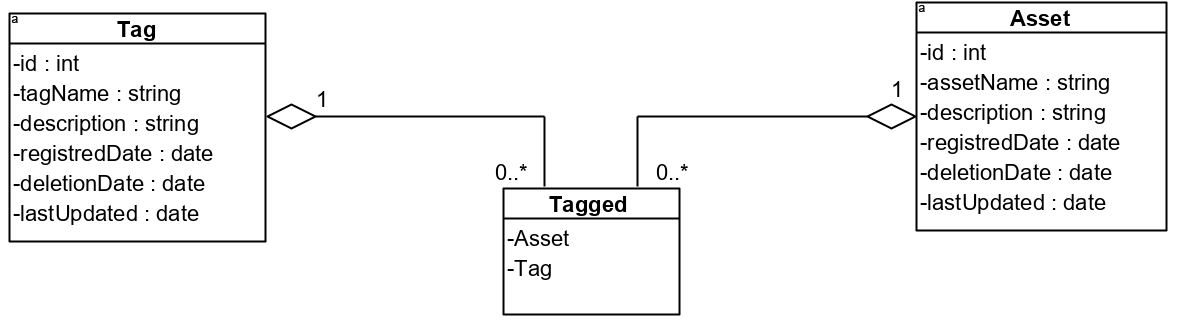
\includegraphics[width=0.8\textwidth]{figures/Structures/TagAssetRelation.PNG}
%     \caption{Overview of the asset class}
%     \label{fig:TagAssetRelation}
% \end{figure}

% \subsubsection{A department contains assets}
% Assets are added to a department, as they are created. An asset belongs to exactly one department, and a department containing multiple assets.

% \begin{figure}[H]
%     \centering
%     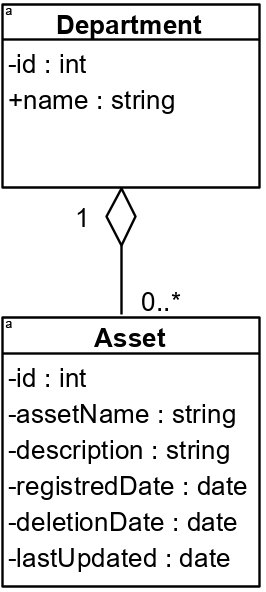
\includegraphics[width=0.2\textwidth]{figures/Structures/AssetDepartmentRelation.PNG}
%     \caption{Overview of the asset class}
%     \label{fig:AssetDepartmentRelation}
% \end{figure}

\subsubsection{Parent tags}
To increase visibility in the system, parent tags are introduced. This is done by adding a connection from the \textit{Tag} class to itself. By doing this, one tag can contain a list of tags, which are seen as its children. A tag can only belong to one other tag or contain a number of tags. This means that there is no single tag that can act as both parent and child. As a product of this, the structure becomes a two level hierarchy (see \autoref{fig:TagHierarchy}).
\todo[inline]{Forklar, at denne funktionalitet er implementeret som attributer på tag, og billeder bare er illustrativt}

\begin{figure}[H]
    \centering
    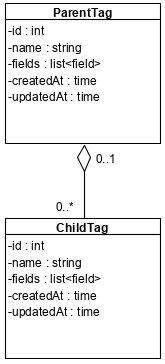
\includegraphics[width=0.35\textwidth]{figures/Structures/TagHierarchy.png}
    \caption{Overview of the structure of the \textit{ParentTag} and \textit{ChildTag} classes}
    \label{fig:TagHierarchy}
\end{figure}

The diagram is purely illustrative, as the implementation of this relation is accomplished through a couple attributes on the tag class. One of the attributes is called \textit{parentId} and contains the ID of the parent of the current tag. If the tag has no parent, this ID is 0.

\subsection{Updated class-diagram}
The additions mentioned above have added up to the following class-diagram, which represents the model component. The \textit{ParentTag} and \textit{ChildTag} classes are simply tags without or with a parent respectively. Therefore the tag has been made abstract and the two tag types are specializations of this abstract class.

% Tags og andre ting skal introduceres inden dette afsnit
\begin{figure}[H]
    \centering
    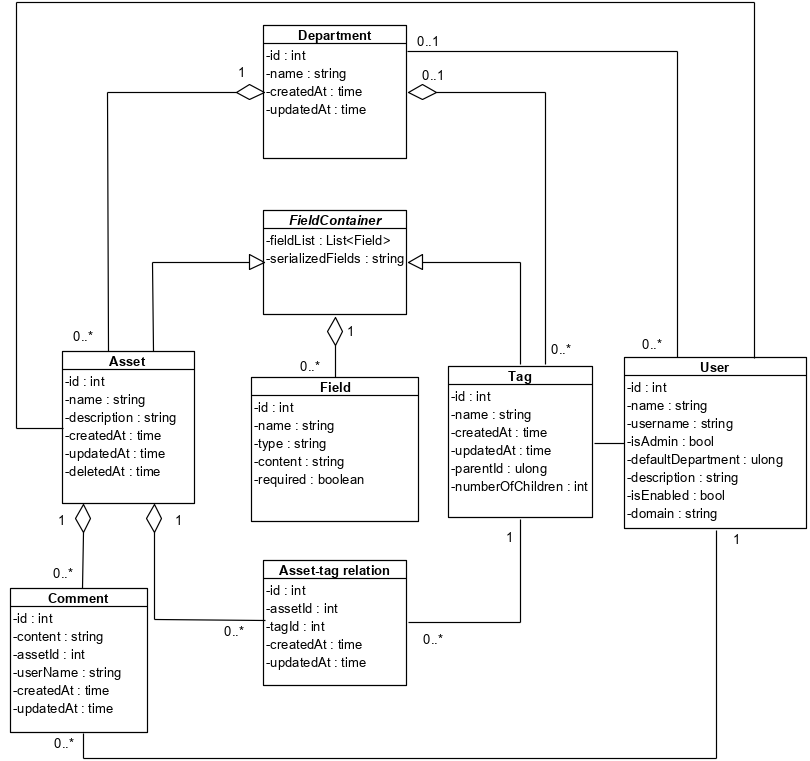
\includegraphics[width=0.9\textwidth]{figures/ClassDiagrams/ModelComponentClassDiagram.png}
    \caption{Class diagram for the model component}
    \label{fig:ModelComponentClassDiagram}
\end{figure}

As illustrated in figure \ref{fig:ModelComponentClassDiagram}, the classes now contain need attributes to represent the information needed for each class. The function component has then been constructed, and operations have been added to the model component, to accommodate for the functions described in the event table (table \ref{ssc:eventtable}) and state charts (section \ref{sc:behavoir}). This has been documented in the next section.